\subsection{Schaltregler}\label{schaltregler}

Gemäss Vorgaben des Auftraggebers wurde das zur Spannungsregelung zuständige Bauteil mittels eines Abwärtswandlers im Form eines Schaltreglers realisiert. Die Ausgangsspannung des Reglers soll vom Controller in Form einer DC-Spannung reguliert werden, sodass der Ausgang der im Mikrocontroller hinterlegten Kennlinie entspricht. 

Gewählt wurde der LT1074CT \colorbox{red}{Hersteller?}, da dieser Ströme bis zu 5A sowie eine maximale Ausgangsspannung von 50V besitzt. Die maximale Eingansspannung beträgt 60V, deutlich mehr als die Spannung des Netzgerätes, welche 24V beträgt.
Des weiteren lässt sich der LT1074CT verhältnismässig einfach mittels eines Feedback-Pins regulieren und die TO-220 Gehäuseform erlaubt eine einfache Montage eines Kühlkörpers.

Auch kann bei Bedarf auf den LT1074HVCT \colorbox{red}{Hersteller?} gewechselt werden. Dieser besitzt nebst den Funktionen des LT1074CT auch noch einen Stromlimit-Pin und einen Stutdown-Pin. Die Strombegrenzung kann mittels Widerstandes auf einen anderen maximalen Ausgangsstrom als die standardmässigen 6A \colorbox{red}{Nicht auch 5A wie oben?} eingestellt werden. Da jedoch der Strom des Netzteils 4.2A beträgt ist eine Begrenzung des Stromes nicht notwendig und  der Shutdown-Pin ist lediglich dazu da, um den Regler abzuschalten, falls eine zu tiefe Spannung vorhanden ist. Da diese zusätzlichen Funktionen für Virtual Sun nicht benötigt werden, ist der LT1074CT jedoch ausreichend. \colorbox{yellow}{Eventuell wären diese Funktionen bei der Weiterentwicklung praktisch (vor allem die Strombegrenzung). Das könnte man im Text noch erwähnen.}

\begin{figure}[h]
\centering
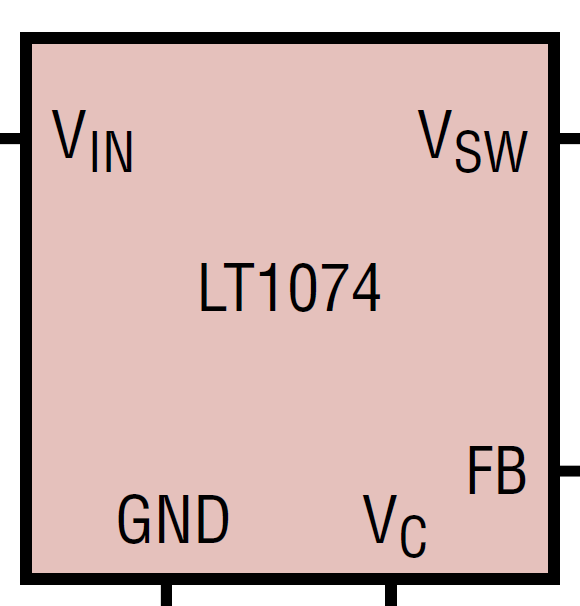
\includegraphics[width=0.2\textwidth]{LTData}%
\caption{Blockschaltbild des LT1074CT.}
\label{fig::LTData}
\end{figure}

Die Schaltung wurde zunächst in LTSpice simuliert und danach auf einer Lochrasterplatine aufgebaut: \colorbox{yellow}{Mach doch die Widerstände mit dem selben Symbol wie bei mir: European Resistor. Dann kannst du die Schaltung als Druckvorschau ausgeben, um den grauen Hintergrund zu vermeiden (oder du sagst mir wo es ist und ich erledige das für dich).}

\begin{figure}[h]
\centering
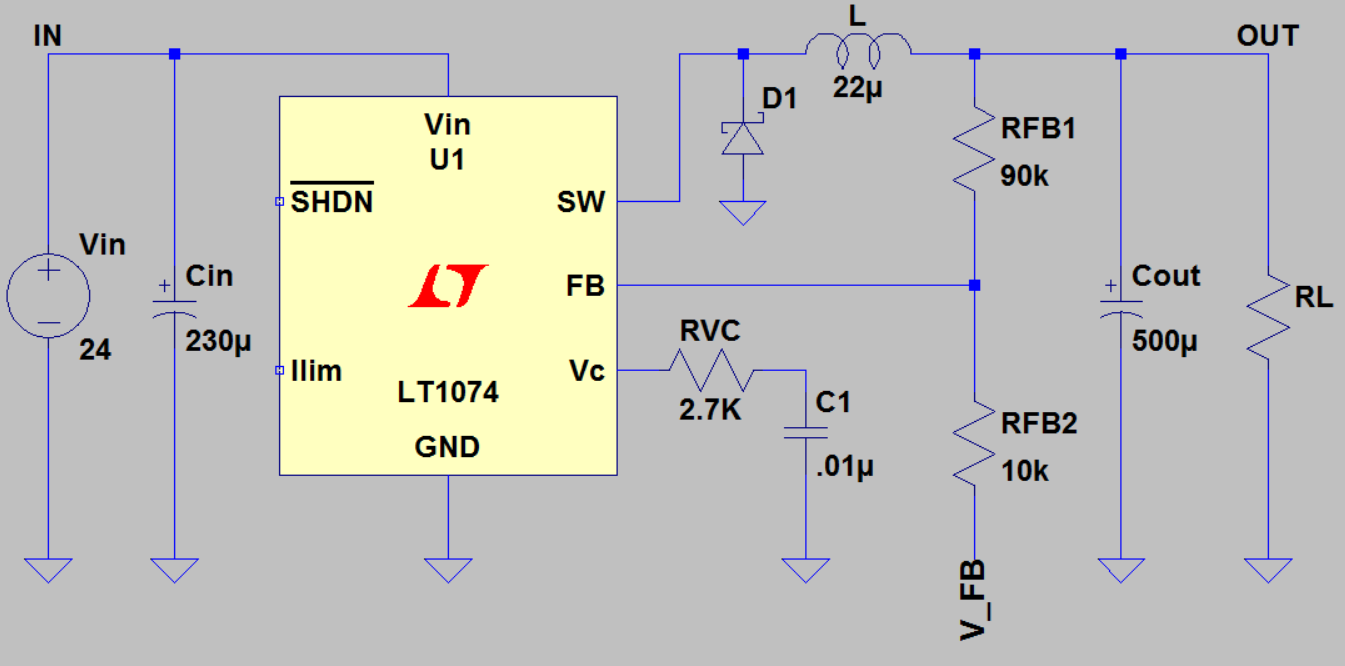
\includegraphics[width=0.8\textwidth]{LTSchemata}%
\caption{Beschaltung des Schaltreglers}%
\label{fig::LTSchemata}%
\end{figure}

Der Widerstand RFB1 wurde mit der folgenden Fromel berechnet: \colorbox{red}{Quelle?}

\[
R_{FB1}=\frac{R_{FB2}\cdot V_{Outmax}}{2.21V}-R_{FB2}
\]

Dabei sind $V_{OutMax} =22$V und $R_{FB2} =10$k$\Omega$, dies ergibt für $R_{FB1} \approx 90$k$\Omega$

Die Spule sowie die Kondensatoren und der Widerstand $R_{Vc}$ wurden gemäss der Appplication Note \colorbox{red}{Quelle!} von Linear Technology dimensioniert und entsprechen damit den Empfehlungen des Herstellers.

Mittels der Spannung $V_{FB}$ kann nun die Ausgangsspannung folgendermassen manipuliert werden:

\[
V_{FB}=2.21\text{V}\cdot\frac{R_{FB1}+R_{FB2}}{R_{FB1}}-V_{out}\cdot\frac{R_{FB2}}{R_{FB1}}
\]

Man sieht sofort, dass bei $V_{FB}=0V$ die Ausgangsspannung maximal wird, das Maximum der Ausgangsspannung wird mit $V_{FB}=2.46V$  erreicht. \colorbox{yellow}{Da kann etwas nicht stimmen...}

Die Funktion dieser Schaltung wurde im Kapitel \ref{subsec:ValRegler} getestet und validiert.